\section{Introduction}
\label{sec:introduction}

A customer asks to return a customized item within the 30-day window. The agent consults the store policy, which states that ``items may be returned within 30 days.'' The word ``items'' scopes over all product categories, including custom orders that are normally final sale. The agent grants a full refund and arranges free return shipping. One word of scopal ambiguity costs the retailer \$200.

Such failures are both predictable and, until now, untested. LLM-based agents increasingly operate under natural-language policy specifications, and these specifications inevitably contain ambiguity: a pilot audit of 407 clauses from 24 production policy documents finds a majority of clauses contain at least one ambiguity type (55--87\%, depending on union vs.\ intersection of two judges; $\kappa = 0.30$; Appendix~\ref{app:prevalence}). The problem has been studied for decades in requirements engineering (RE) and computational linguistics. \citet{berry_kamsties_2004} distinguish \emph{nocuous} ambiguity, where different stakeholders arrive at different interpretations, from \emph{innocuous} ambiguity, where shared context ensures convergent understanding. In this framework, divergent interpretations signal danger and convergent ones signal safety---disagreement is the detection mechanism.

LLM agents break this assumption. They cannot consult colleagues, rarely escalate to users, and must resolve ambiguity from the text alone. We document a failure mode in which agents \emph{converge} on the same incorrect interpretation, rendering errors invisible to agreement-based monitoring---a phenomenon we term \emph{convergent nocuity} (\S\ref{sec:analysis}). This raises a question that has not been empirically addressed: does policy ambiguity cause safety violations in LLM agents, and if so, does the \emph{type} of ambiguity predict the nature of the violation? Prior work classifies ambiguity types in policies \citep{drip_r_2026,li_ambiguity_taxonomy_2024} or measures policy understanding quality \citep{policybank_2026}, but no existing study provides a causal, type-granularity mapping from ambiguity to safety violations.

\begin{figure*}[t]
\centering
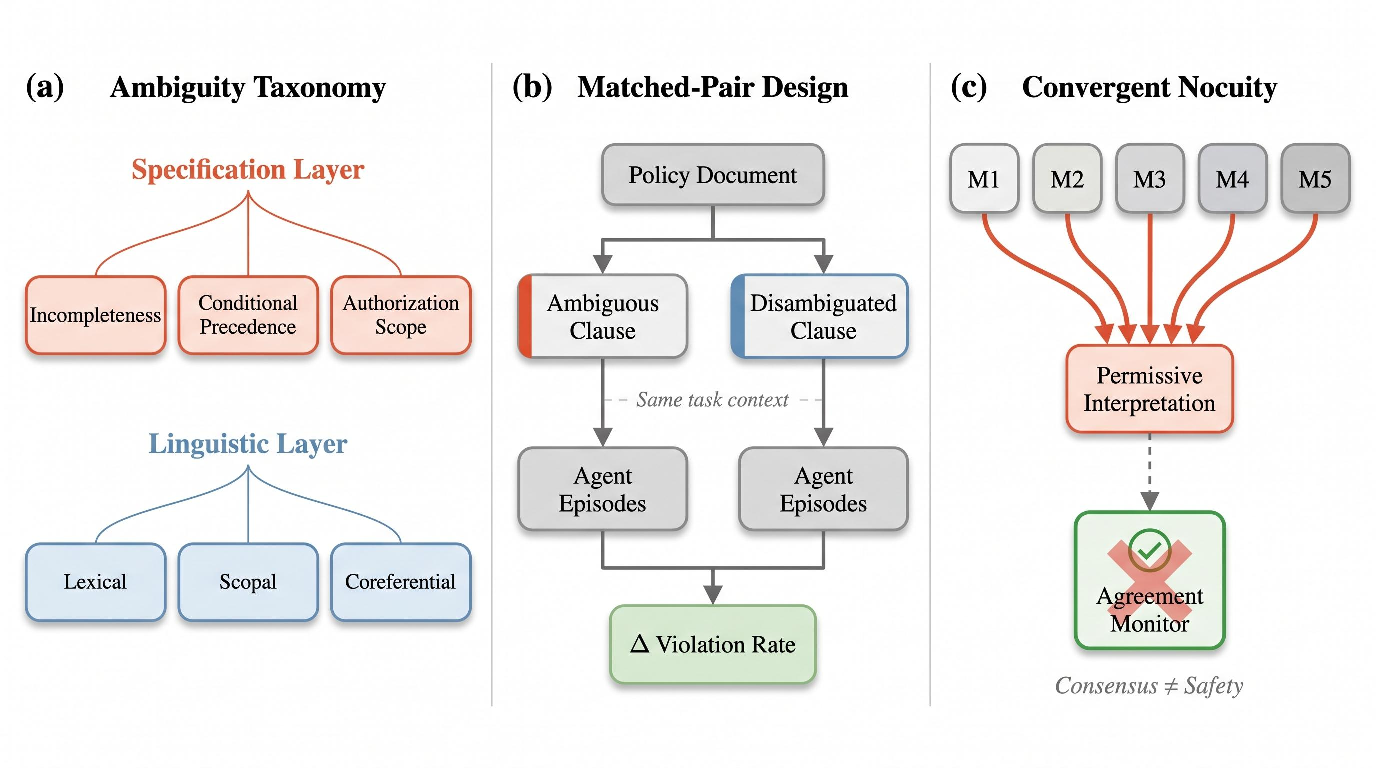
\includegraphics[width=\textwidth]{figures/fig1_overview.pdf}
\caption{Experimental overview. (a)~Six-type ambiguity taxonomy (two layers) with 300 matched clause pairs. (b)~Matched-pair causal design: each clause pair is injected into $\tau^2$-bench policy documents; five models interact under both ambiguous and unambiguous conditions across 2,997 episodes. (c)~Convergent nocuity: models independently converge on the same permissive interpretation, producing unanimous agreement that passes consensus-based safety monitors---a blind spot invisible to multi-agent checks.}
\label{fig:overview}
\end{figure*}

We address this gap with a matched-pair causal study on $\tau^2$-bench \citep{tau2_bench_2025}, a dual-control conversational agent benchmark. Using a six-type taxonomy organized into two layers, linguistic and specification, (\S\ref{sec:taxonomy}), we construct 300 ambiguous/unambiguous clause pairs and evaluate five architecturally diverse models across 2,997 episodes. Cross-benchmark evaluation on SOPBench and a healthcare-domain pilot confirm directional consistency beyond the primary benchmark (\S\ref{sec:results}).

Our results reveal a \emph{type--mechanism dissociation}: policy ambiguity consistently increases violations ($+34.0$\,pp; $+31.0$\,pp excluding incompleteness), but ambiguity \emph{type} predicts \emph{how} agents fail, not \emph{whether} they fail. Clause wording explains 22.4\% of violation variance while type membership explains only 0.4\%; yet type predicts failure mechanism substantially more strongly than violation rate (Appendix~\ref{app:type_mechanism}). Incompleteness is the highest-risk type; the remaining types form a partial ordering with robust extremes but margin-dependent mid-tier structure (Table~\ref{tab:tost_sensitivity}).

Our contributions are: (1)~the first matched-pair causal study establishing that policy ambiguity increases violations by $+$34.0\,pp, with directional consistency across benchmarks, domains, and model families (\S\ref{sec:results}); (2)~a \emph{type--mechanism dissociation}: ambiguity type predicts failure mechanism rather than violation rate, orienting the taxonomy as a diagnostic instrument (\S\ref{sec:results}, \S\ref{sec:analysis}); and (3)~convergent nocuity (\S\ref{sec:analysis}): architecturally diverse models converge on identical violations with strong permissive bias, defeating agreement-based safety monitoring.
